The simulation based optimization tool provides a plug-in system where different derivative free optimization (DFO) solvers can be used with FOQUS. Several solvers are provided with FOQUS. The CMA-ES solver \citep{Hansen_2006} is a good global derivative free optimization (DFO) solver. The NLopt library provides access to several DFO solvers \citep{Johnson_2015}. SLSQP and BFGS from the Scipy module are also provided \citep{Scipy_2015}. Since FOQUS does not generally have access to derivative information the Scipy solvers rely on finite difference approximations, and should only be used with well-behaved functions. Due to convergence tolerances in process simulators, finite difference approximations may not be good for many of FOQUS's intended applications.

CMA-ES offers a restart feature, which can be used to resume an optimization if it is interrupted for any reason. Other solvers may use an auto-save feature, which does not provide the ability to restart, but will allow optimization to start from the best solution found up to the point the optimization was interrupted.  Samples making up the population in CMA-ES can be run in parallel. The NLopt and Scipy plugins do not offer parallel computing for standard optimization. For any solver, parallel computation can be used for parameter estimation and optimization under uncertainty, where multiple flowsheet evaluations go into an objective function calculation.
%The subsection is numbered incorrectly. Goes from 3.01 to 3.1, should be 3.1, 3.2, etc. Please correct.
\section{Problem Set Up}

See Chapter \ref{chpt.flowsheet} for information about setting up a flowsheet in FOQUS. Once the flowsheet has been set up and tested, an optimization problem can be added. FOQUS allows multiple flowsheet evaluations to be used to calculate a single objective function value. This allows FOQUS to do parameter estimation and scenario based optimization under uncertainty.  There are three types of variables used in the optimization problem: (1) fixed variables do not change during the optimization, (2) decision variables are modified by the optimization algorithm to find the best value of the objective function, and (3) sample variables, which are used to construct the multiple flowsheet evaluations that can go into an objective calculation. If no sample variables are defined, each objective function value will be based on a single flowsheet evaluation.  Figure \ref{fig.opt.problem.variables} shows the \textbf{\underline{Variables}} tab selection form.

\begin{figure}[H]
	\begin{center}
		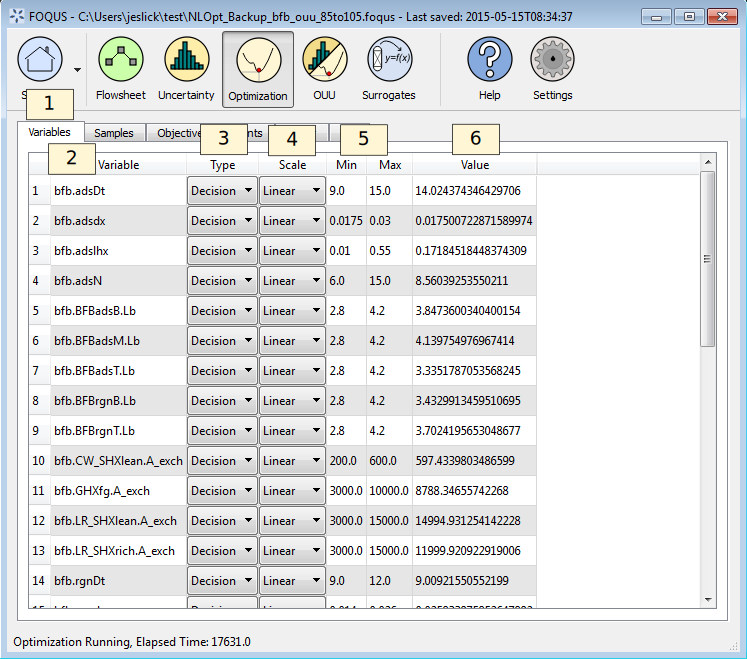
\includegraphics[scale=0.55]{Chapt_optimization/figs/opt_problem_variables}
		\caption{Optimization Variable Selection}
		\label{fig.opt.problem.variables}
	\end{center}
\end{figure}

\begin{enumerate}
	\item The \bu{Variables} tab contains the form for variables selection.
	\item The \textbf{\underline{Variable}} column shows the name of input variables in the flowsheet. If a variable is set by a connection to another variable through an edge, it is not shown in the table. The format for a variable name is \{Node Name\}.\{Variable Name\}.
	\item The \textbf{\underline{Type}} column allows the variables to be assigned as one of three types (1) fixed, (2) decision, or (3) sample.
	\item The \textbf{\underline{Scale}} column allows the scaling method to be set for each variable. Decision variables must be scaled. Scaling is ignored for other variables. In the FOQUS example files, there is a scaling spreadsheet that provides a demonstration of the different scaling methods. The upper and lower bound are used in the scaling calculations. Regardless of the scaling method, the optimizer sees the decision variables as running from 0 at their minimum to 10 at their maximum. 
	\item The \textbf{\underline{Min}} and \textbf{\underline{Max}} columns are used to define the upper and lower bounds for the variables. FOQUS requires that all optimization problems be bounded.
	\item The \textbf{\underline{Value}} column provides the starting point for the optimization. How the starting point is used depends on the optimization method. The starting point for sample variables is irrelevant. Fixed variables will remain at their starting point during the optimization.
\end{enumerate}

The sample variables define a set of samples that will be used to calculate an objective function. For each objective function, the decision variables are fixed at values set by the optimization solver, and the flowsheet is evaluated for each row on the sample table. The results of the samples can be used to calculate the objective function. Using the \textbf{\underline{Samples}} tab is optional. If no sample variables are set, each objective function value will be based on a single simulation. Figure \ref{fig.opt.problem.samples} shows the Samples table form.   

\begin{figure}[H]
	\begin{center}
		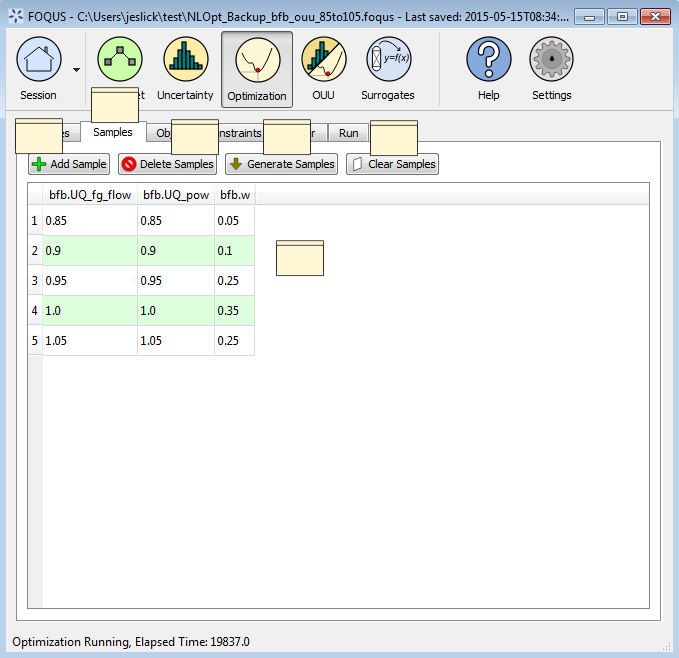
\includegraphics[scale=0.55]{Chapt_optimization/figs/opt_problem_samples}
		\caption{Optimization Sample Table}
		\label{fig.opt.problem.samples}
	\end{center}
\end{figure}

\begin{enumerate}
	\item The \bu{Samples} tab contains the table used to define samples for objective function calculations. If there are no sample variables, the table should be empty.
	\item \bu{Add Sample} adds a row to the Samples table.
	\item \bu{Delete Samples} deletes the selected rows from the Samples table.
	\item \bu{Generate Samples} opens a dialog box that provides a selection of methods to generate samples or read samples from a file.
	\item \bu{Clear Samples} clears the Samples table.
\end{enumerate}

Once the variables and (optionally) samples have been selected, the objective function and constraints can be defined. FOQUS is set up to handle multi-objective optimization, but no multi-objective optimization plug-ins are currently provided in the FOQUS installer, so some of the options may seem to be extraneous. There are two methods for entering the objective function and constraints into FOQUS: (1) Simple Python expressions and (2) a more extensive Python function. Python expressions are easier and sufficient for most cases. If the objective function is complicated it may be necessary to write a Python function, which can be as complex as needed.

The variables used in the Python code for the objective function or constraints are stored in two Python dictionaries, ``f'' for outputs and ``x'' for inputs. There are two ways to index the dictionaries depending on whether or not sample variables are used. For an input variable with sampling, the indexing is \texttt{x[Sample Index]['Node Name']['Variable Name'][Time Step Index]}. If no sample variables are defined, the sample index is not needed, so the indexing would be, \texttt{x['Node Name']['Variable Name'][Time Step]}.  Node Name and Variable Name are strings so they should be in quotes. The sample and time step indexes are integers. For steady state simulations, the time step should be 0.

Figure \ref{fig.opt.problem.objective1} shows the form for entering the objective function and constraints as Python expressions.

\begin{figure}[H]
	\begin{center}
		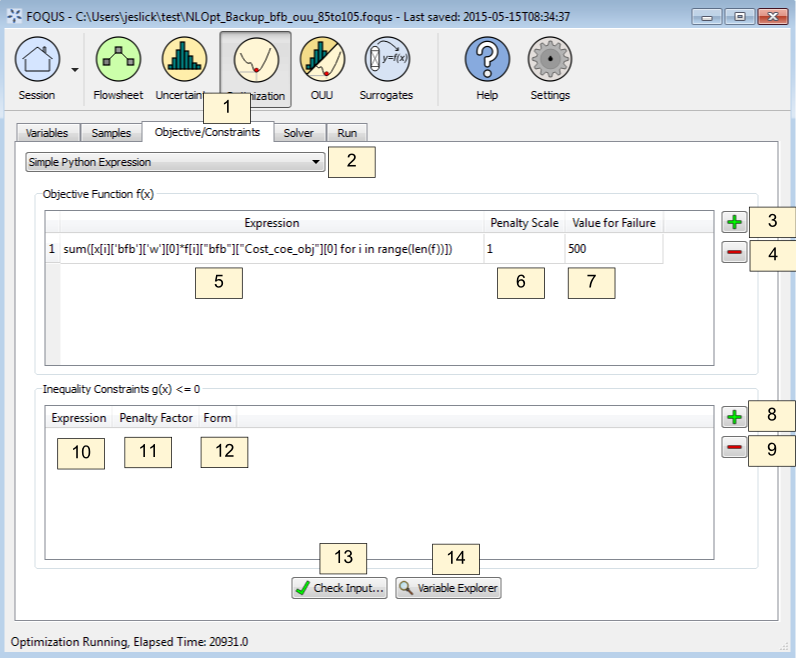
\includegraphics[scale=0.55]{Chapt_optimization/figs/opt_problem_objective1}
		\caption{Optimization Simple Objective Function}
		\label{fig.opt.problem.objective1}
	\end{center}
\end{figure}

\begin{enumerate}
	\item The \bu{Objective/Constraints} tab contains the form used to enter the objective function and constraints.
	\item The drop-down list enables the selection of either the ``Simple Python Expression'' or ``Custom Python'' form of the objective function.
	\item \bu{+} adds an objective function to the table. The solvers currently available are single objective and will only use the first objective function.
	\item \bu{-} removes the selected objective from the table.
	\item The Python expression for the objective function can be entered in the \textbf{\underline{Expression}} column.
	\item The \textbf{\underline{Penalty Scale}} column is intended for use with multi-objective solvers and allows the constraint violation penalty to be applied differently to objective functions with different magnitudes.
	\item The \textbf{\underline{Value for Failure}} column contains the value to be assigned to the objective function if the objective cannot be evaluated for any reason. The value should be higher than the expected highest value for a successful objective.
	\item \bu{+} adds an inequality constraint.
	\item \bu{-} removes selected inequality constraints.
	\item The inequality constraints are in the form $g(\mathbf{x}) \leq 0$. The \textbf{\underline{Expression}} column contains the Python expression for $g(\mathbf{x})$.
	\item The \textbf{\underline{Penalty Factor}} contains the coefficient $a$ used in calculating the penalty for a constraint violation, see Equations \ref{eq.linear.constriant} to \ref{eq.step.constriant}.
	\item The \textbf{\underline{Form}} column contains a selection of different methods to calculate a constraint penalty.
	\item \bu{Check Input} checks the problem for any mistakes that can be detected before running the optimization.
	\item \bu{Variable Explorer} enables the user to browse the variables in the simulation. They can be copied and pasted into the Python expression. The variables are provided without the sample index.
\end{enumerate}

The calculations for each type of constraint penalty are given in Equations \ref{eq.linear.constriant} to \ref{eq.step.constriant}.

\begin{equation}\label{eq.linear.constriant}
	\text{Linear penalty form:  }p_i = 
	\begin{cases}
		0 & \text{if } g_i(\mathbf{x}) \leq 0\\
		a \times g_i(\mathbf{x}) & \text{if } g_i(\mathbf{x}) > 0
	\end{cases}
\end{equation}

\begin{equation}\label{eq.quadratic.constriant}
\text{Quadratic penalty form:  }p_i = 
\begin{cases}
0 & \text{if } g_i(\mathbf{x}) \leq 0\\
a \times g_i(\mathbf{x})^2 & \text{if } g_i(\mathbf{x}) > 0
\end{cases}
\end{equation}

\begin{equation}\label{eq.step.constriant}
\text{Step penalty form:  }p_i = 
\begin{cases}
0 & \text{if } g_i(\mathbf{x}) \leq 0\\
a & \text{if } g_i(\mathbf{x}) > 0
\end{cases}
\end{equation}

If the Simple Python Expression method of entering the objective function does not offer enough flexibility, the Custom Python method can be used. The Custom Python method enables the user to enter the objective calculation as a Python function, which also should include any required constraint penalties.

Figure \ref{fig.opt.problem.objective2} shows the Custom Python objective form. The top text box provides instructions for writing a custom objective function. The bottom text box provides a place to enter Python code. The numpy and math modules have been imported and are available as numpy and math. To use the Custom Python objective, the user must define a function called ``onjfunc(x, f, fail).''  The three arguments are: (1) ``x'' is the dictionary of input variables, (2) ``f'' is the dictionary of output variables, and (3) ``fail'' is a boolean vector that indicates whether a particular sample calculation has failed. The ``objfunc'' function should return three values: (1) a list of objective function values for multi-objective optimization (in most cases with single objective optimization this will be a list with one value), (2) a list of constraint violations, and (3) the total constraint penalty. The constraint violation and penalty information are only used for debugging, so they are not required. It is safe to return [0] and 0 for the constraint information regardless of whether a constraint penalty has been added to the objective.
 
\begin{figure}[H]
	\begin{center}
		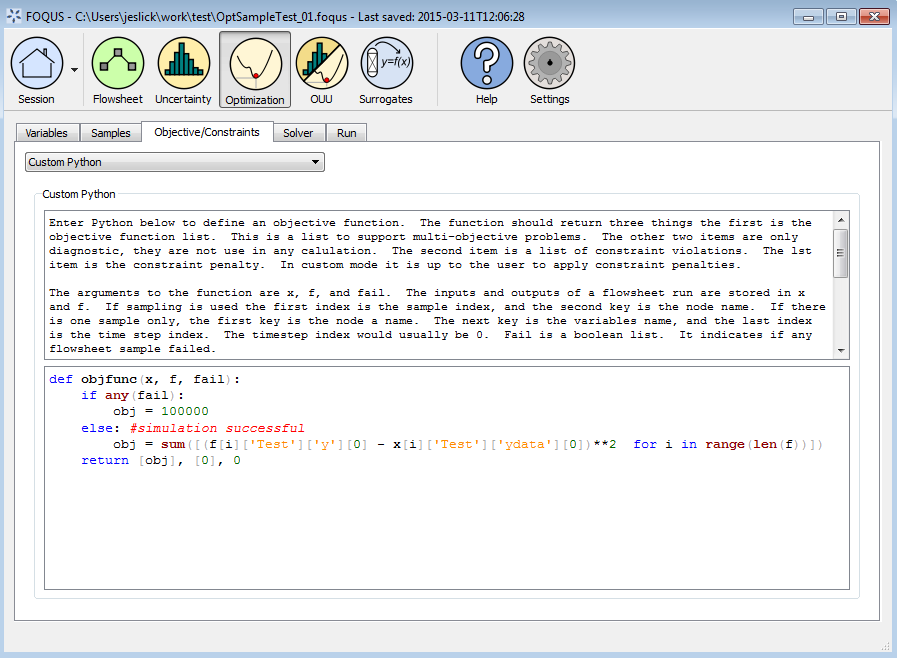
\includegraphics[scale=0.55]{Chapt_optimization/figs/opt_problem_objective2}
		\caption{Custom  Objective Function}
		\label{fig.opt.problem.objective2}
	\end{center}
\end{figure}

The code in Figure \ref{fig.opt.problem.objective2_code} provides an example of a custom objective function for parameter estimation. The objective function minimizes the sum of the differences between simulation and empirical data. In this case the decision variables would be model parameters. The first line defines a function with three arguments. The ``x'' and ``f'' arguments are the input and output variables. The variable indexing is explained in the simple objective function section.  The ``fail'' argument is a boolean vector where element ``i'' is true if sample ``i'' failed. If there are no sample variables, ``fail'' will only have one element.

The ``if'' in the function determines if any flowsheet evaluation failed, and assigns a bad objective function value if so. If all the flowsheet evaluations where successful, the results are used to calculate the objective function. In the objective function calculation, Python list comprehension is used to calculate the sum of squared errors. In this case, no constraint penalty is needed. The objective function is returned as a list with only one element. The last two return values are debugging information for constraints. In this case, the ``zeros'' are just place holders and have no real utility.

\begin{figure}[H]
\begin{small}
\begin{verbatim}
def objfunc(x, f, fail):
    if any(fail): # any simulation failed
        obj = 100000
    else: #simulations successful
        obj=sum([(f[i]['Test']['y'][0] - x[i]['Test']['ydata'][0])**2\
          for i in range(len(f))])
    return [obj], [0], 0
\end{verbatim}
\end{small}
\caption{Custom  Objective Function Code}
\label{fig.opt.problem.objective2_code}
\end{figure}

\section{Solver Options}\label{sec.opt.solver.options}

The \bu{Solver} tab in the \textbf{\underline{Optimization}} button tool enables the selection of the DFO method and setting of solver parameters. Figure \ref{fig.opt.solver.form} illustrates the solver form.
\begin{figure}[H]
	\begin{center}
		\includegraphics[scale=0.55]{Chapt_optimization/figs/opt_solver_form}
		\caption{Optimization Solver Form}
		\label{fig.opt.solver.form}
	\end{center}
\end{figure}

Elements of the solver form are:
\begin{enumerate}
	\item \bu{Select Solver} drop-down list, which enables the user to select from available DFO solvers.
	\item \bu{Description} text box provides a description of the selected DFO solver.
	\item \bu{Solver Options} table contains the solver settings and a description of each option. The settings depend on the selected plug-in.
\end{enumerate}

\section{Running Optimization}

The optimization monitor is displayed under the \bu{Run} tab in the \textbf{\underline{Optimization}} button tool. The optimization monitor, illustrated in Figure \ref{fig.opt.run.form}, is used to monitor the progress of the optimization as it runs.

\begin{figure}[H]
	\begin{center}
		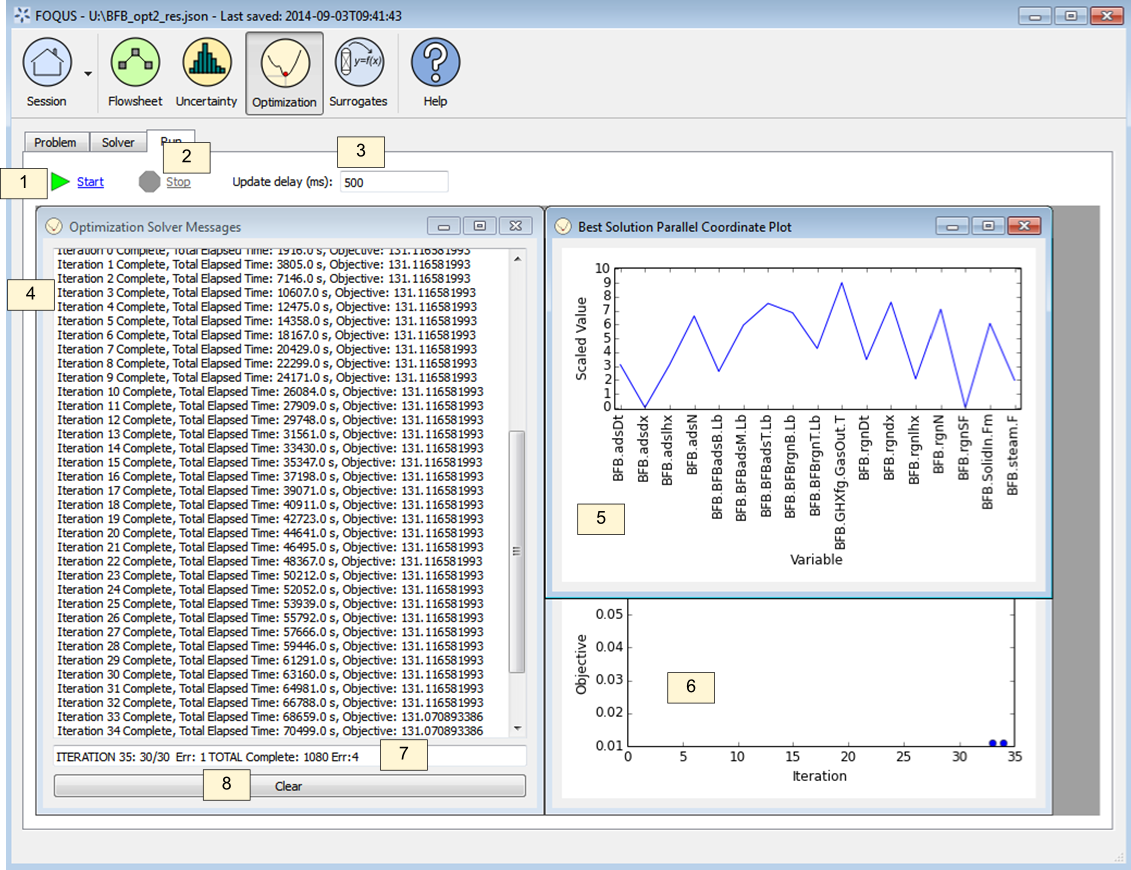
\includegraphics[scale=0.50]{Chapt_optimization/figs/opt_run_form}
		\caption{Optimization Monitor Form}
		\label{fig.opt.run.form}
	\end{center}
\end{figure}

Elements of the optimization monitor are:
\begin{enumerate}
	\item \bu{Start} starts the optimization.
	\item \bu{Stop} stops the optimization. The best solution found when optimization is stopped is stored in the flowsheet.
	\item \bu{Update delay} is how often the user interface communicates with the optimization thread to update the display.
	\item \bu{Optimization Solver Messages} displays output from the optimization solver.
	\item \bu{Best Solution Parallel Coordinate Plot} displays the values of the decision variables scaled. This plot is helpful in identifying when variables are at, or near, their bounds.
	\item \bu{Objective Function Plot} displays the objective function value at each iteration.
	\item \bu{Status Box} displays the current iteration, how many samples have been run, how many sample were successful, and how many failed.
	\item \bu{Clear} deletes solver messages from the solve message box.
\end{enumerate}

As the optimization runs, the FOQUS flowsheet is updated to include the best solution found. If sampling is used, the first sample in the best objective function is stored in the flowsheet. If for any reason the optimization terminates, the best solution found is available in the flowsheet. The results for all flowsheet evaluations done for the optimization are available in the Results table in the Flowsheet Editor.

